\chapter{Installation of Simile}
In this chapter we will show how to install the tools we used for implementing Simile. First we will start installing the CI Server Jenkins and explain how to configure it. Then, we will continue with installing Simile Jenkins plugin. After that we will explain how to configure Simile Jenkins plugin using the test project.

\section{Installation of Jenkins}
In this section we will explain how to install Jenkins CI server using Docker.

\subsection{Docker}
For installing Jenkins, we will use Docker containers and in this subsection we will explain how to install it in different platform such as macOS and Linux.

\subsubsection{Docker on macOS}
For macOS we will use Docker for Mac tool. This is an integrated, easy-to-deploy environment for building, assembling, and shipping applications from a Mac. Moreover, it is a native Mac application architected from scratch, with a native user interface and auto-update capability, deeply integrated with OS X native virtualization, Hypervisor Framework, networking and file system, making it faster and more reliable than previous ways of getting Docker on a Mac \citep{Docker}.

First we will download the tool from the following link: \url{https://download.docker.com/mac/stable/Docker.dmg}.\\

After downloading the \textit{dmg} image, double-click on it and you will see something like figure \ref{fig:docker-mac-01}. When you get that image, drag and drop the Docker icon to the Applications folder. After that, go to Applications folder and double click on Docker application.

\begin{figure}[ht]
	\centering
    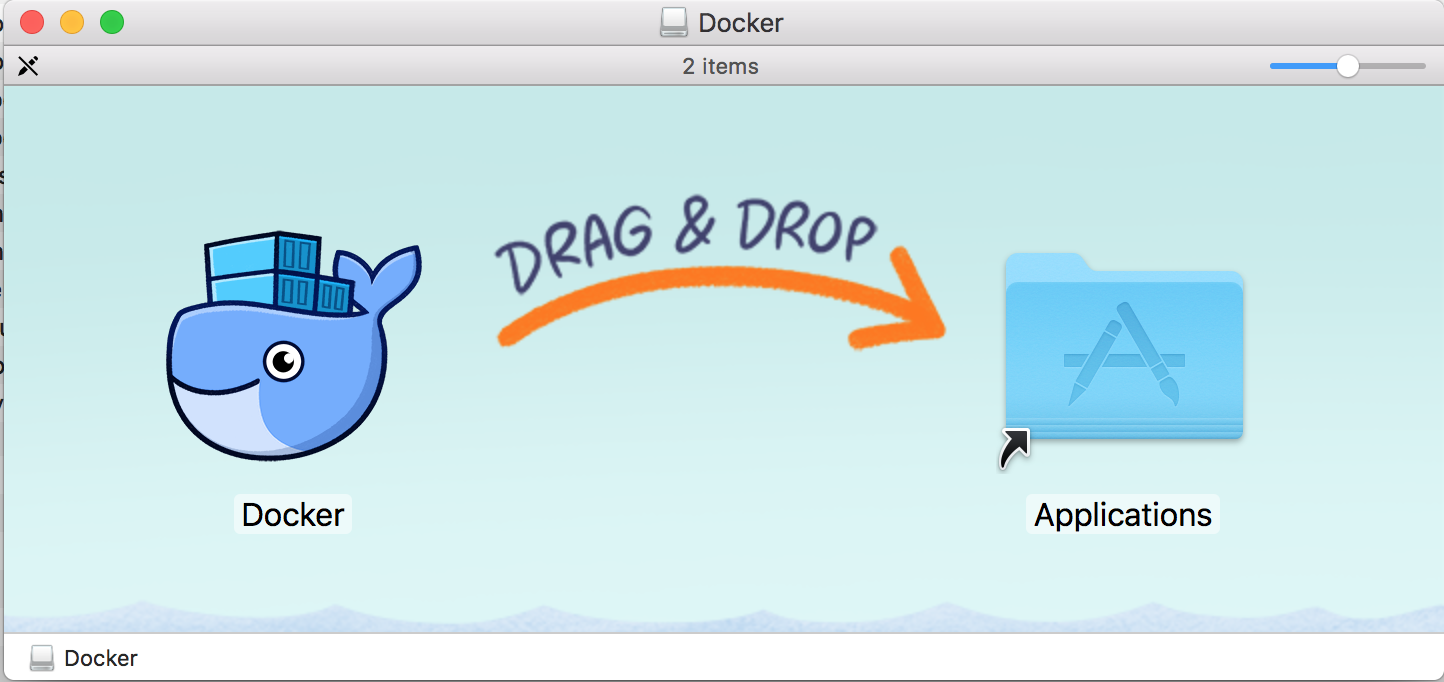
\includegraphics[width=\textwidth]{grafiken/docker-01}
    \caption{Docker for Mac installation}
    \label{fig:docker-mac-01}
\end{figure}

\subsubsection{Docker on Linux}
In this section we will explain how to install Docker in Linux, specifically in Debian (Jessie). For other distros please refer to Docker documentation\footnote{https://docs.docker.com/engine/installation/linux/ (accessed: 21.01.2017)}.

First of all we need to update the repositories.

\begin{minted}[linenos,
               numbersep=5pt,
               frame=lines,
               framesep=2mm]{bash}
$ sudo apt-get udpate
\end{minted}

Then we need to install the packages to allow \textit{apt} to use repositories iver HTTPS.

\begin{minted}[linenos,
               numbersep=5pt,
               frame=lines,
               framesep=2mm]{bash}
$ sudo apt-get install apt-transport-https \
                       ca-certificates \
                       software-properties-common
\end{minted}

Then we add the official Docker's GPG key.

\begin{minted}[linenos,
               numbersep=5pt,
               frame=lines,
               framesep=2mm]{bash}
$ curl -fsSL https://yum.dockerproject.org/gpg | sudo apt-key add -
\end{minted}

Finally we add the stable repository of Docker and update repositories.

\begin{minted}[linenos,
               numbersep=5pt,
               frame=lines,
               framesep=2mm]{bash}
$ sudo add-apt-repository \
       "deb https://apt.dockerproject.org/repo/ \
       debian-$(lsb_release -cs) \
       main"
$ sudo apt-get update
\end{minted}

Once we added the new repositories, we update the repository list.

\begin{minted}[linenos,
               numbersep=5pt,
               frame=lines,
               framesep=2mm]{bash}
$ sudo apt-get update
\end{minted}

Then we install docker.

\begin{minted}[linenos,
               numbersep=5pt,
               frame=lines,
               framesep=2mm]{bash}
$ sudo apt-get -y install docker-engine
\end{minted}

After the installation is done we can make a little test to be sure that everything was installed correctly. The following command will download a test image and runs it in a container. Once it is running will print an informational message and exits.

\begin{minted}[linenos,
               numbersep=5pt,
               frame=lines,
               framesep=2mm]{bash}
$ sudo docker run hello-world
\end{minted}

\subsection{Jenkins in Docker}
Open a terminal on your mac and enter the following command to download the Jenkins image for Docker.

\begin{minted}[linenos,
               numbersep=5pt,
               frame=lines,
               framesep=2mm]{bash}
$ docker pull jenkins
  Using default tag: latest
  latest: Pulling from library/jenkins

  # some irrelevant output was remove
  Digest: sha256:5046434030be395ec977c98e11...
  Status: Downloaded newer image for jenkins:latest
\end{minted}

Then, we just need to run the Jenkins image with the following command.

\begin{minted}[linenos,
               numbersep=5pt,
               frame=lines,
               framesep=2mm,
               breakanywhere]{bash}
$ docker run -p 8080:8080 -p 50000:50000 jenkins
  # some irrelevant output was remove
  *************************************************************

  Jenkins initial setup is required. An admin user has been 
  created and a password generated.
  Please use the following password to proceed to installation:

  95199411f1894bfa97e937147c41aa62 # IMPORTANT, default admin pass

  This may also be found at: /var/jenkins_home/secrets/initial.
 
  *************************************************************
  # some irrelevant output was removed
  Jan 19, 2017 8:28:05 AM hudson.model.AsyncPeriodicWork$1 run
  INFO: Finished Download metadata. 25,312 ms
\end{minted}

After that, open the following URL \url{http://localhost:8080} and you should see some like figure \ref{fig:jenkins-01}.

\begin{figure}[H]
	\centering
    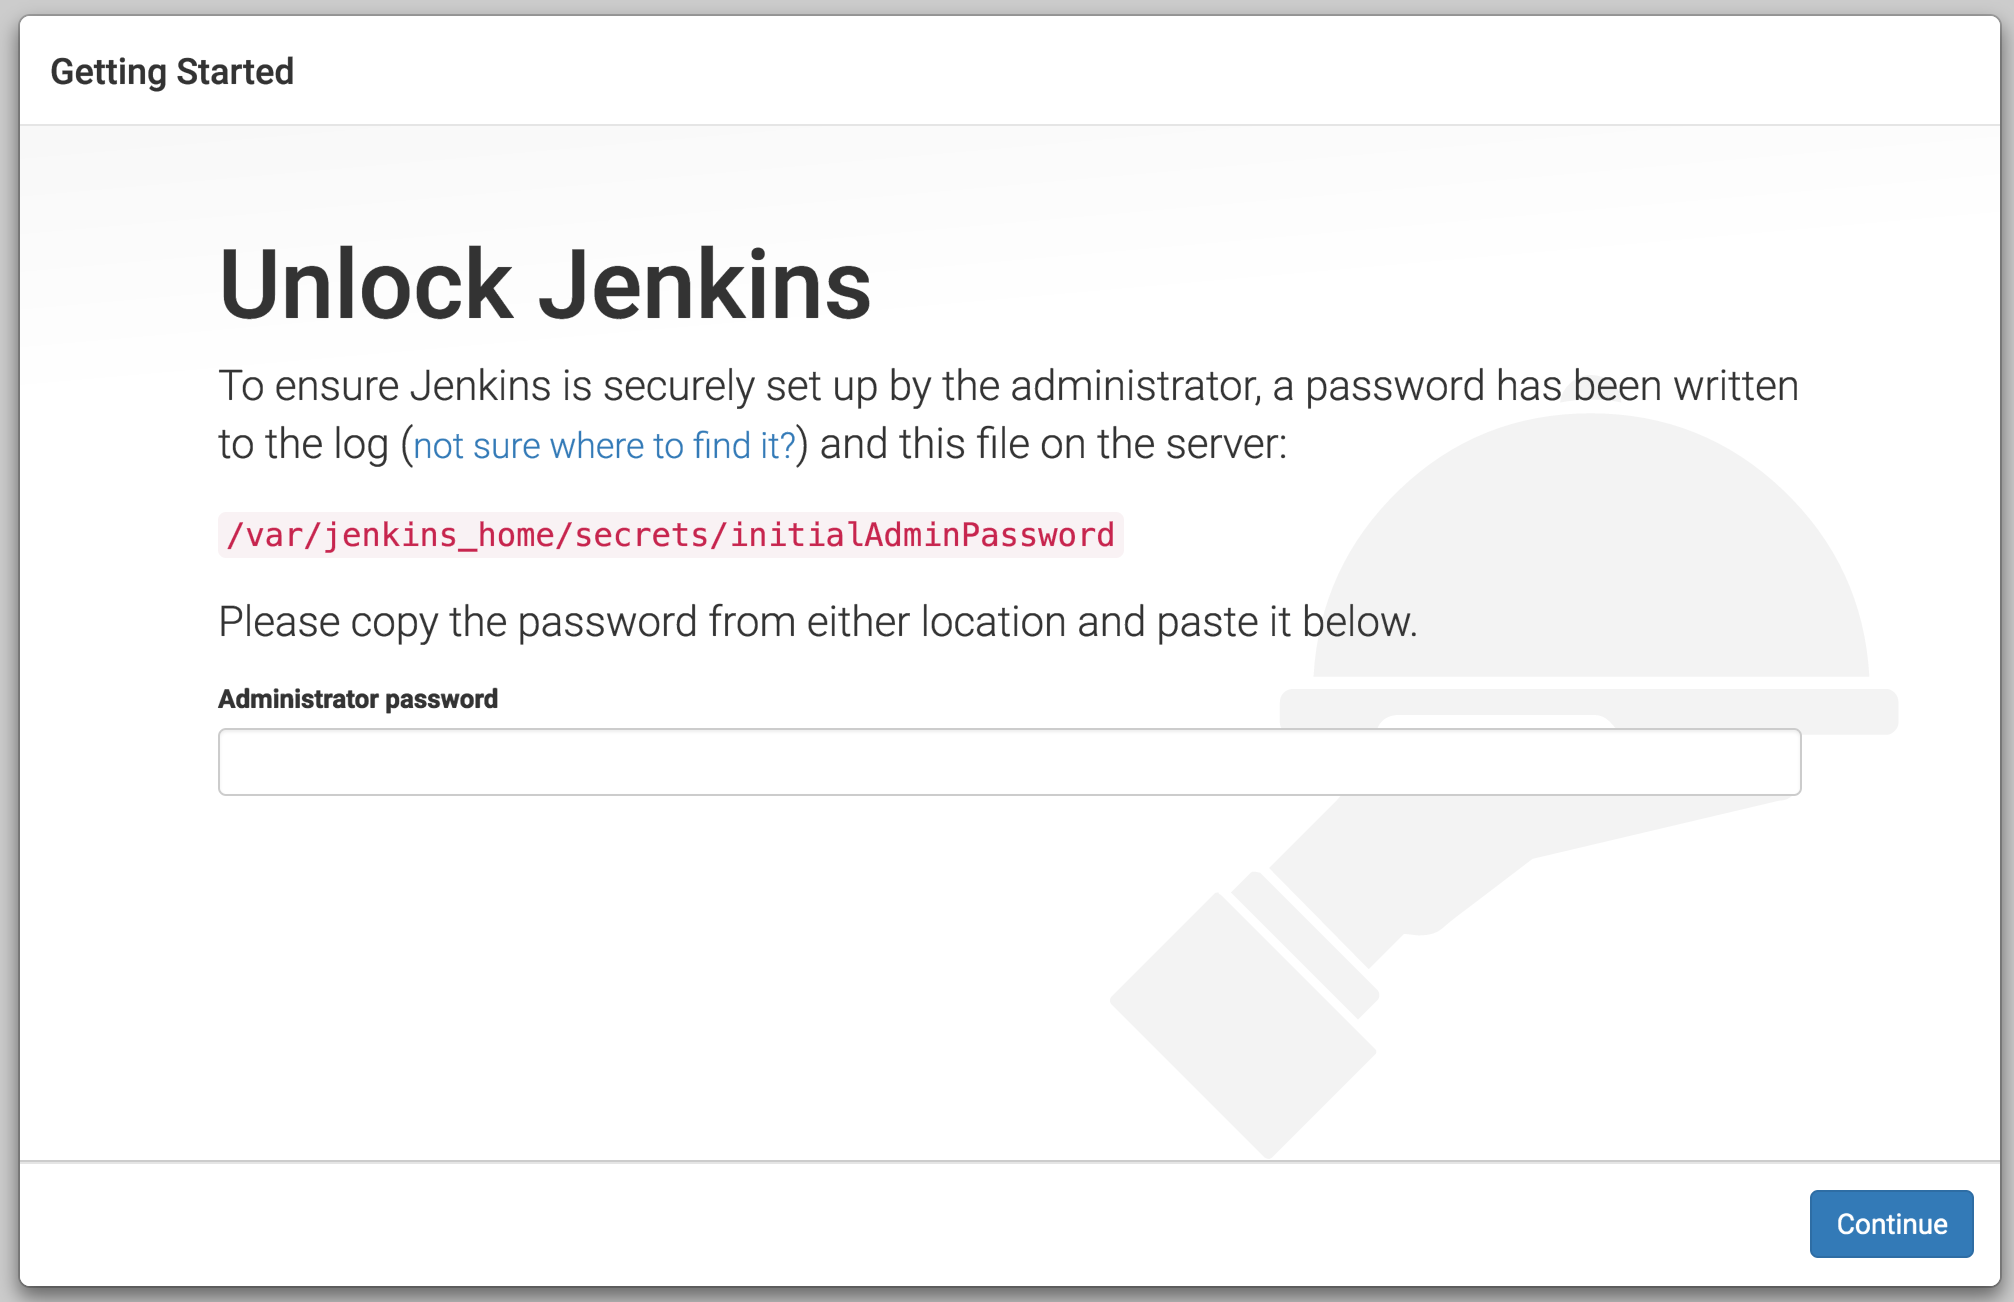
\includegraphics[width=0.7\textwidth]{grafiken/jenkins-01}
    \caption{First page of Jenkins setup}
    \label{fig:jenkins-01}
\end{figure}

There enter the password generated by Jenkins and that appeared in the logs, and then click on continue.

In the folowing page click on \textit{Install suggested plugins} like the figure \ref{fig:jenkins-02}.

\begin{figure}[H]
	\centering
    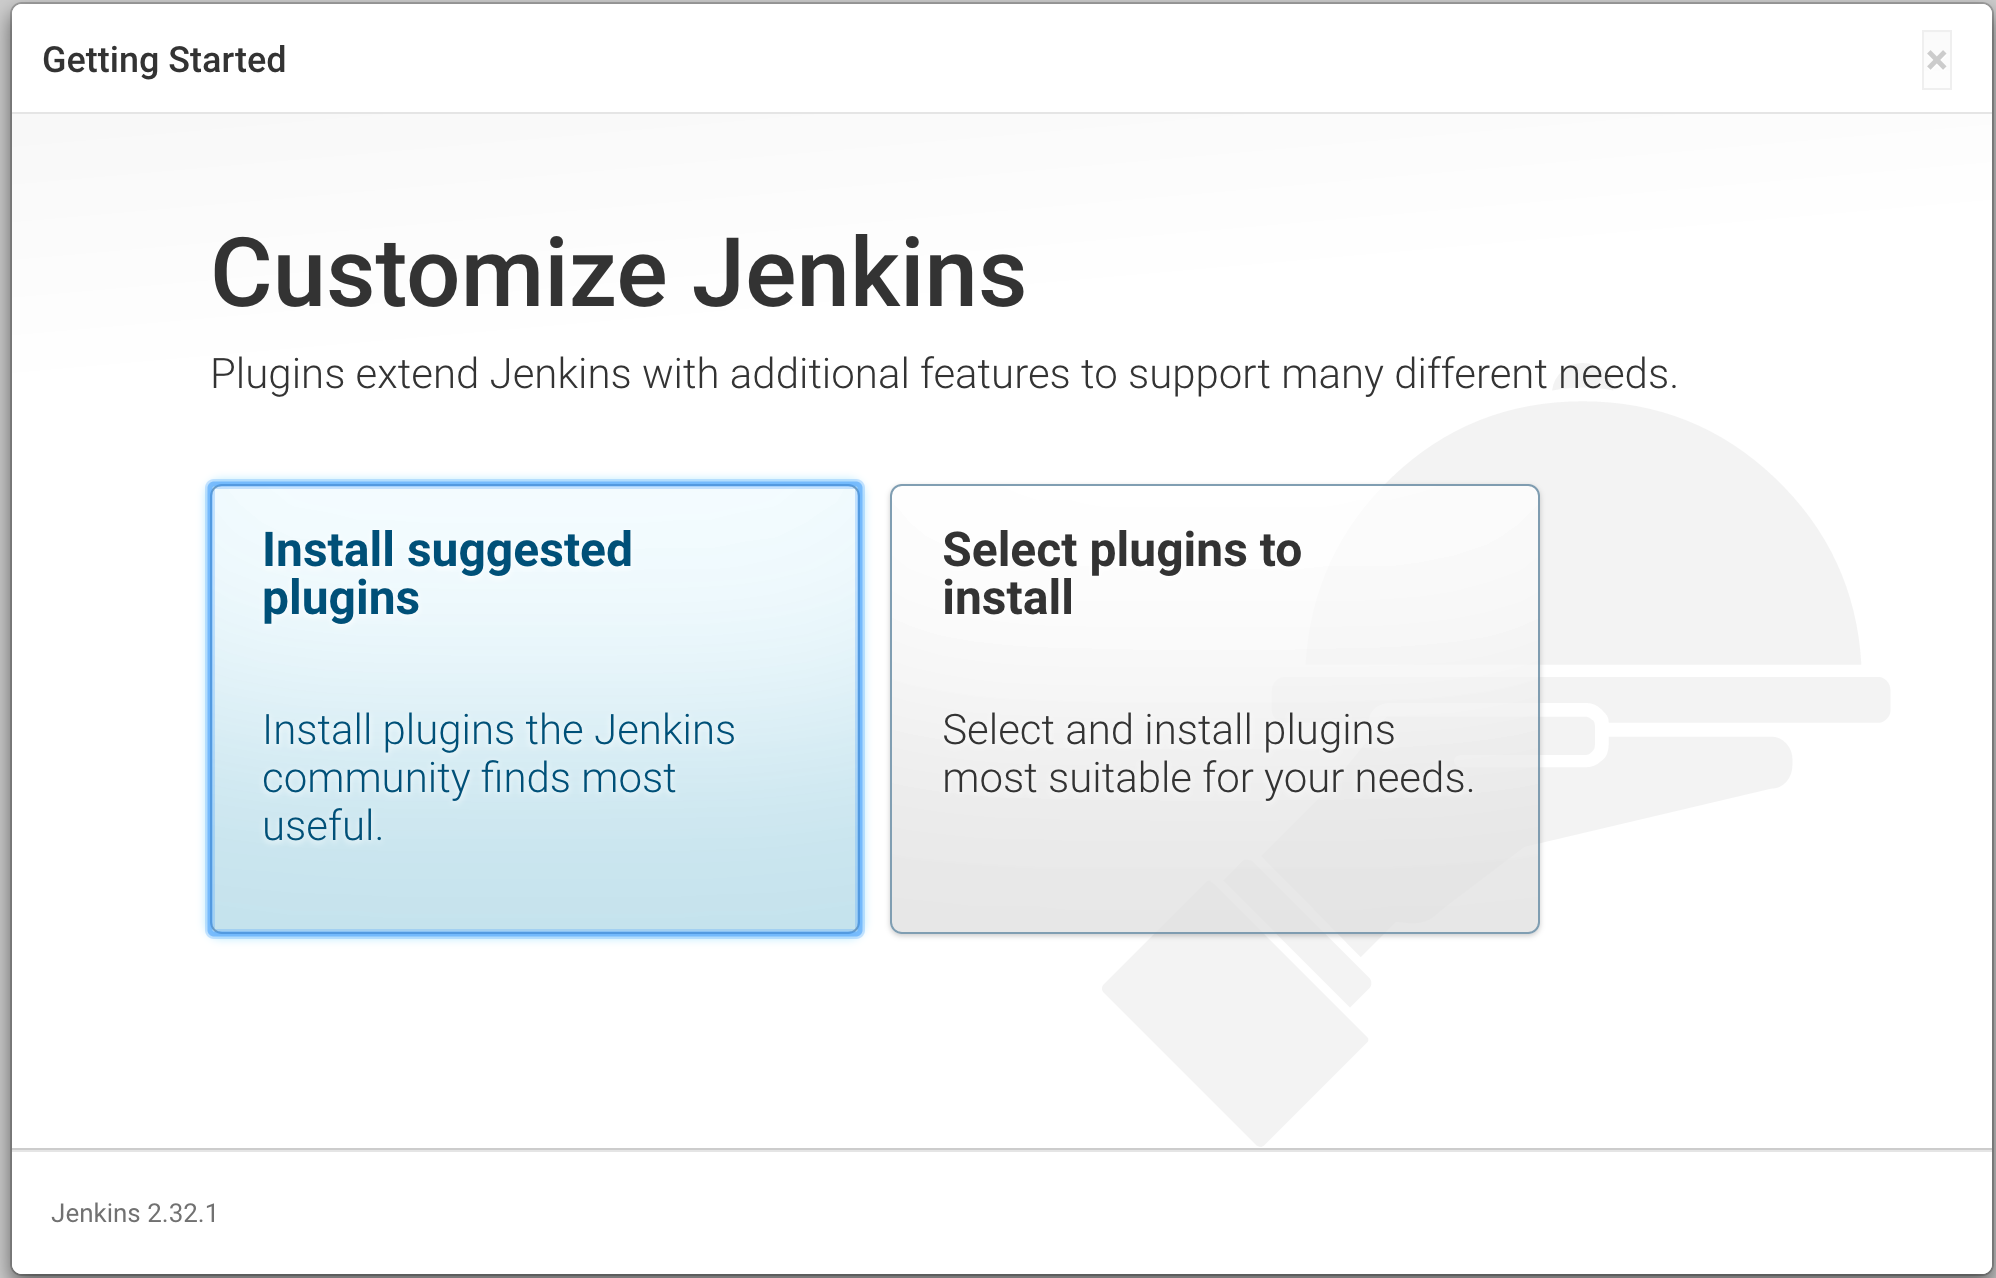
\includegraphics[width=0.8\textwidth]{grafiken/jenkins-02}
    \caption{Second page of Jenkins setup}
    \label{fig:jenkins-02}
\end{figure}

Then you should see something like the figure \ref{fig:jenkins-03}. Here we just need to wait untill the plugins installation finish.

\begin{figure}[H]
	\centering
    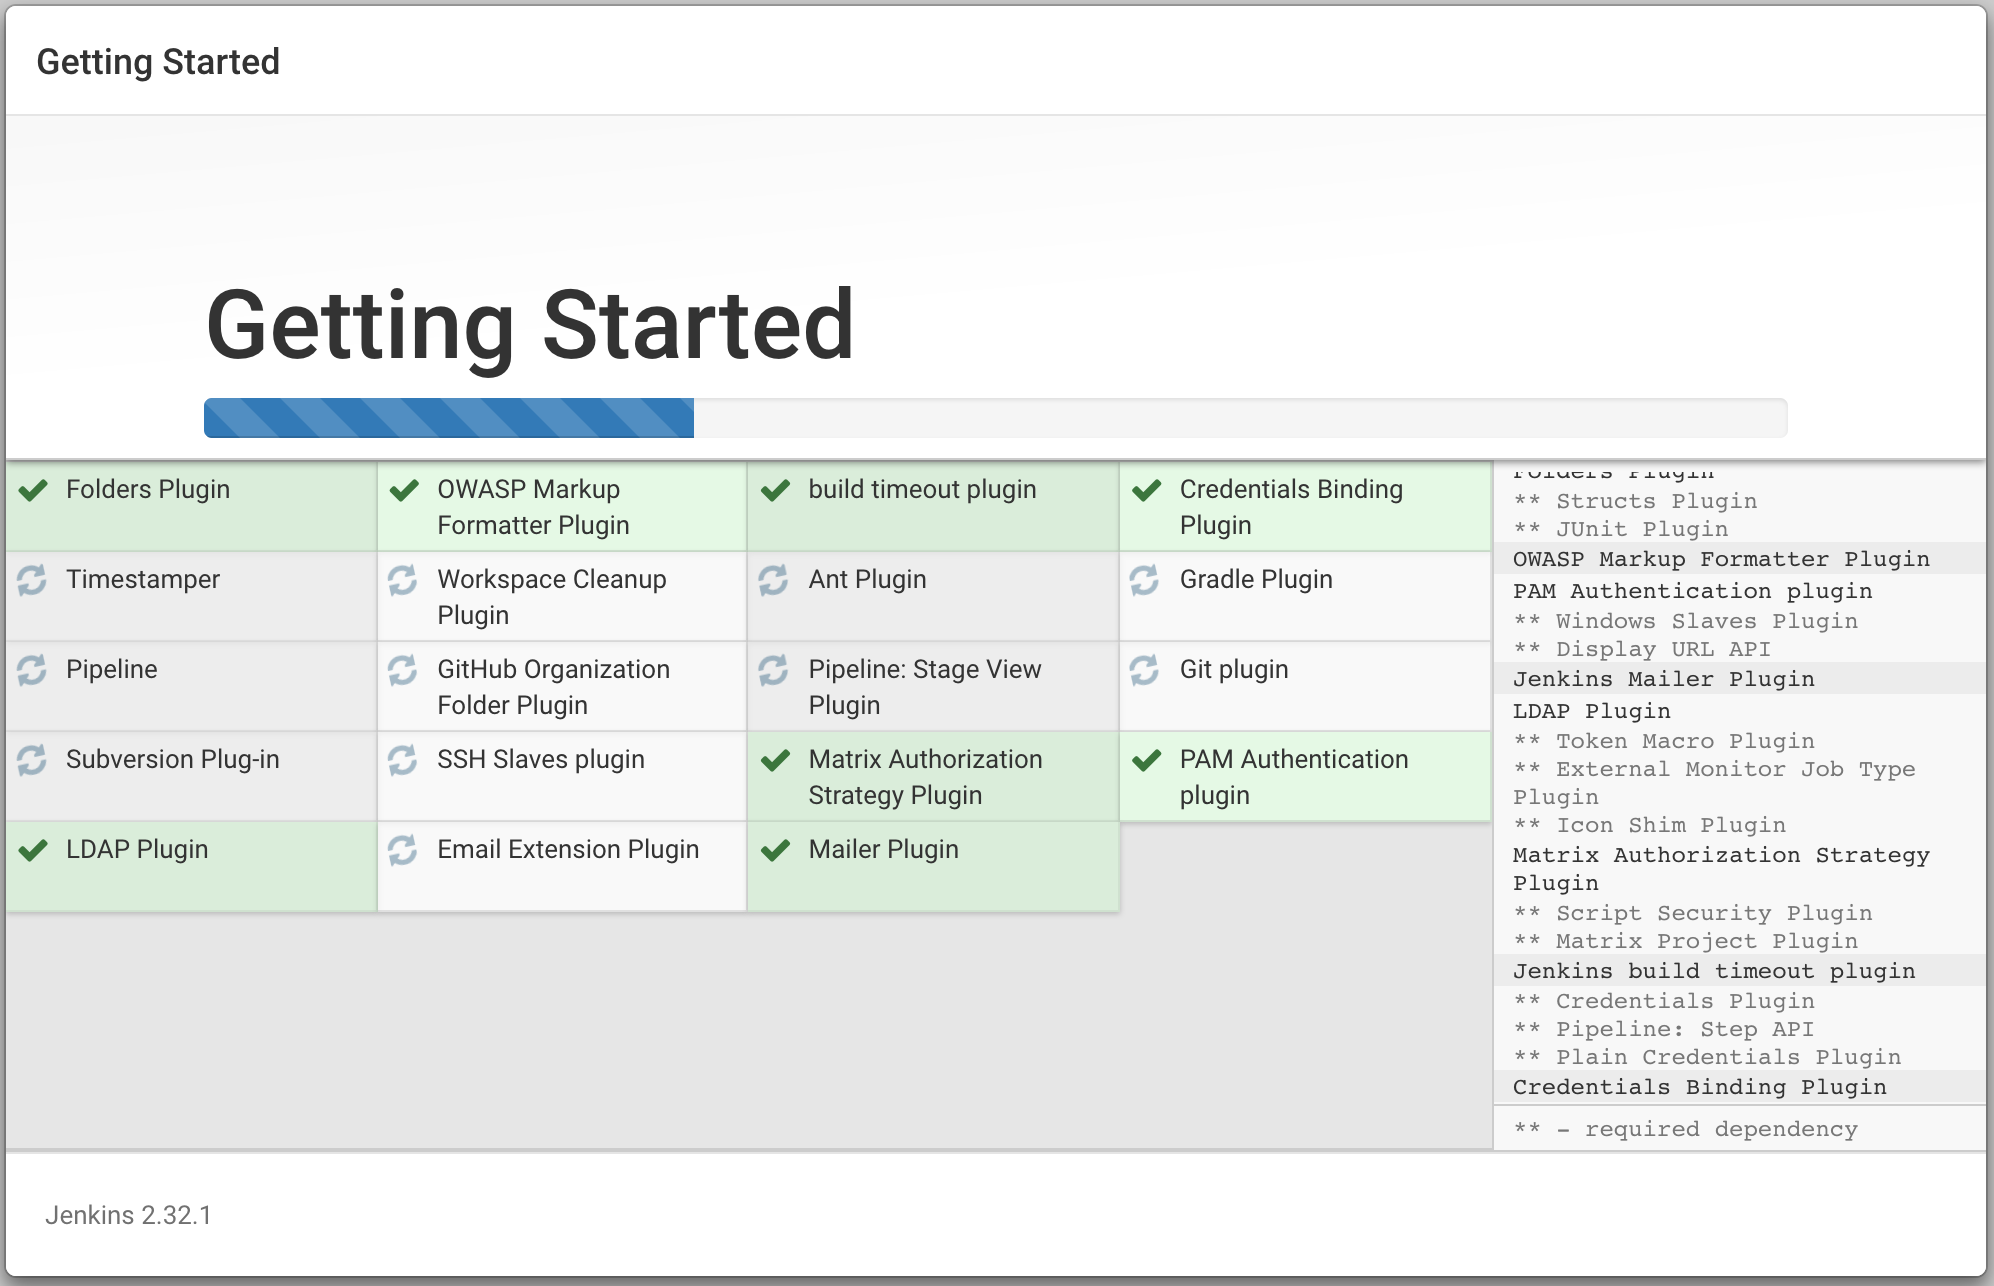
\includegraphics[width=0.8\textwidth]{grafiken/jenkins-03}
    \caption{Third page of Jenkins setup}
    \label{fig:jenkins-03}
\end{figure}

After the installation of plugins is done, click on \textit{Continue as admin} or create custom admin user. Then you should see the home page of Jenkins (figure )

\begin{figure}[H]
	\centering
    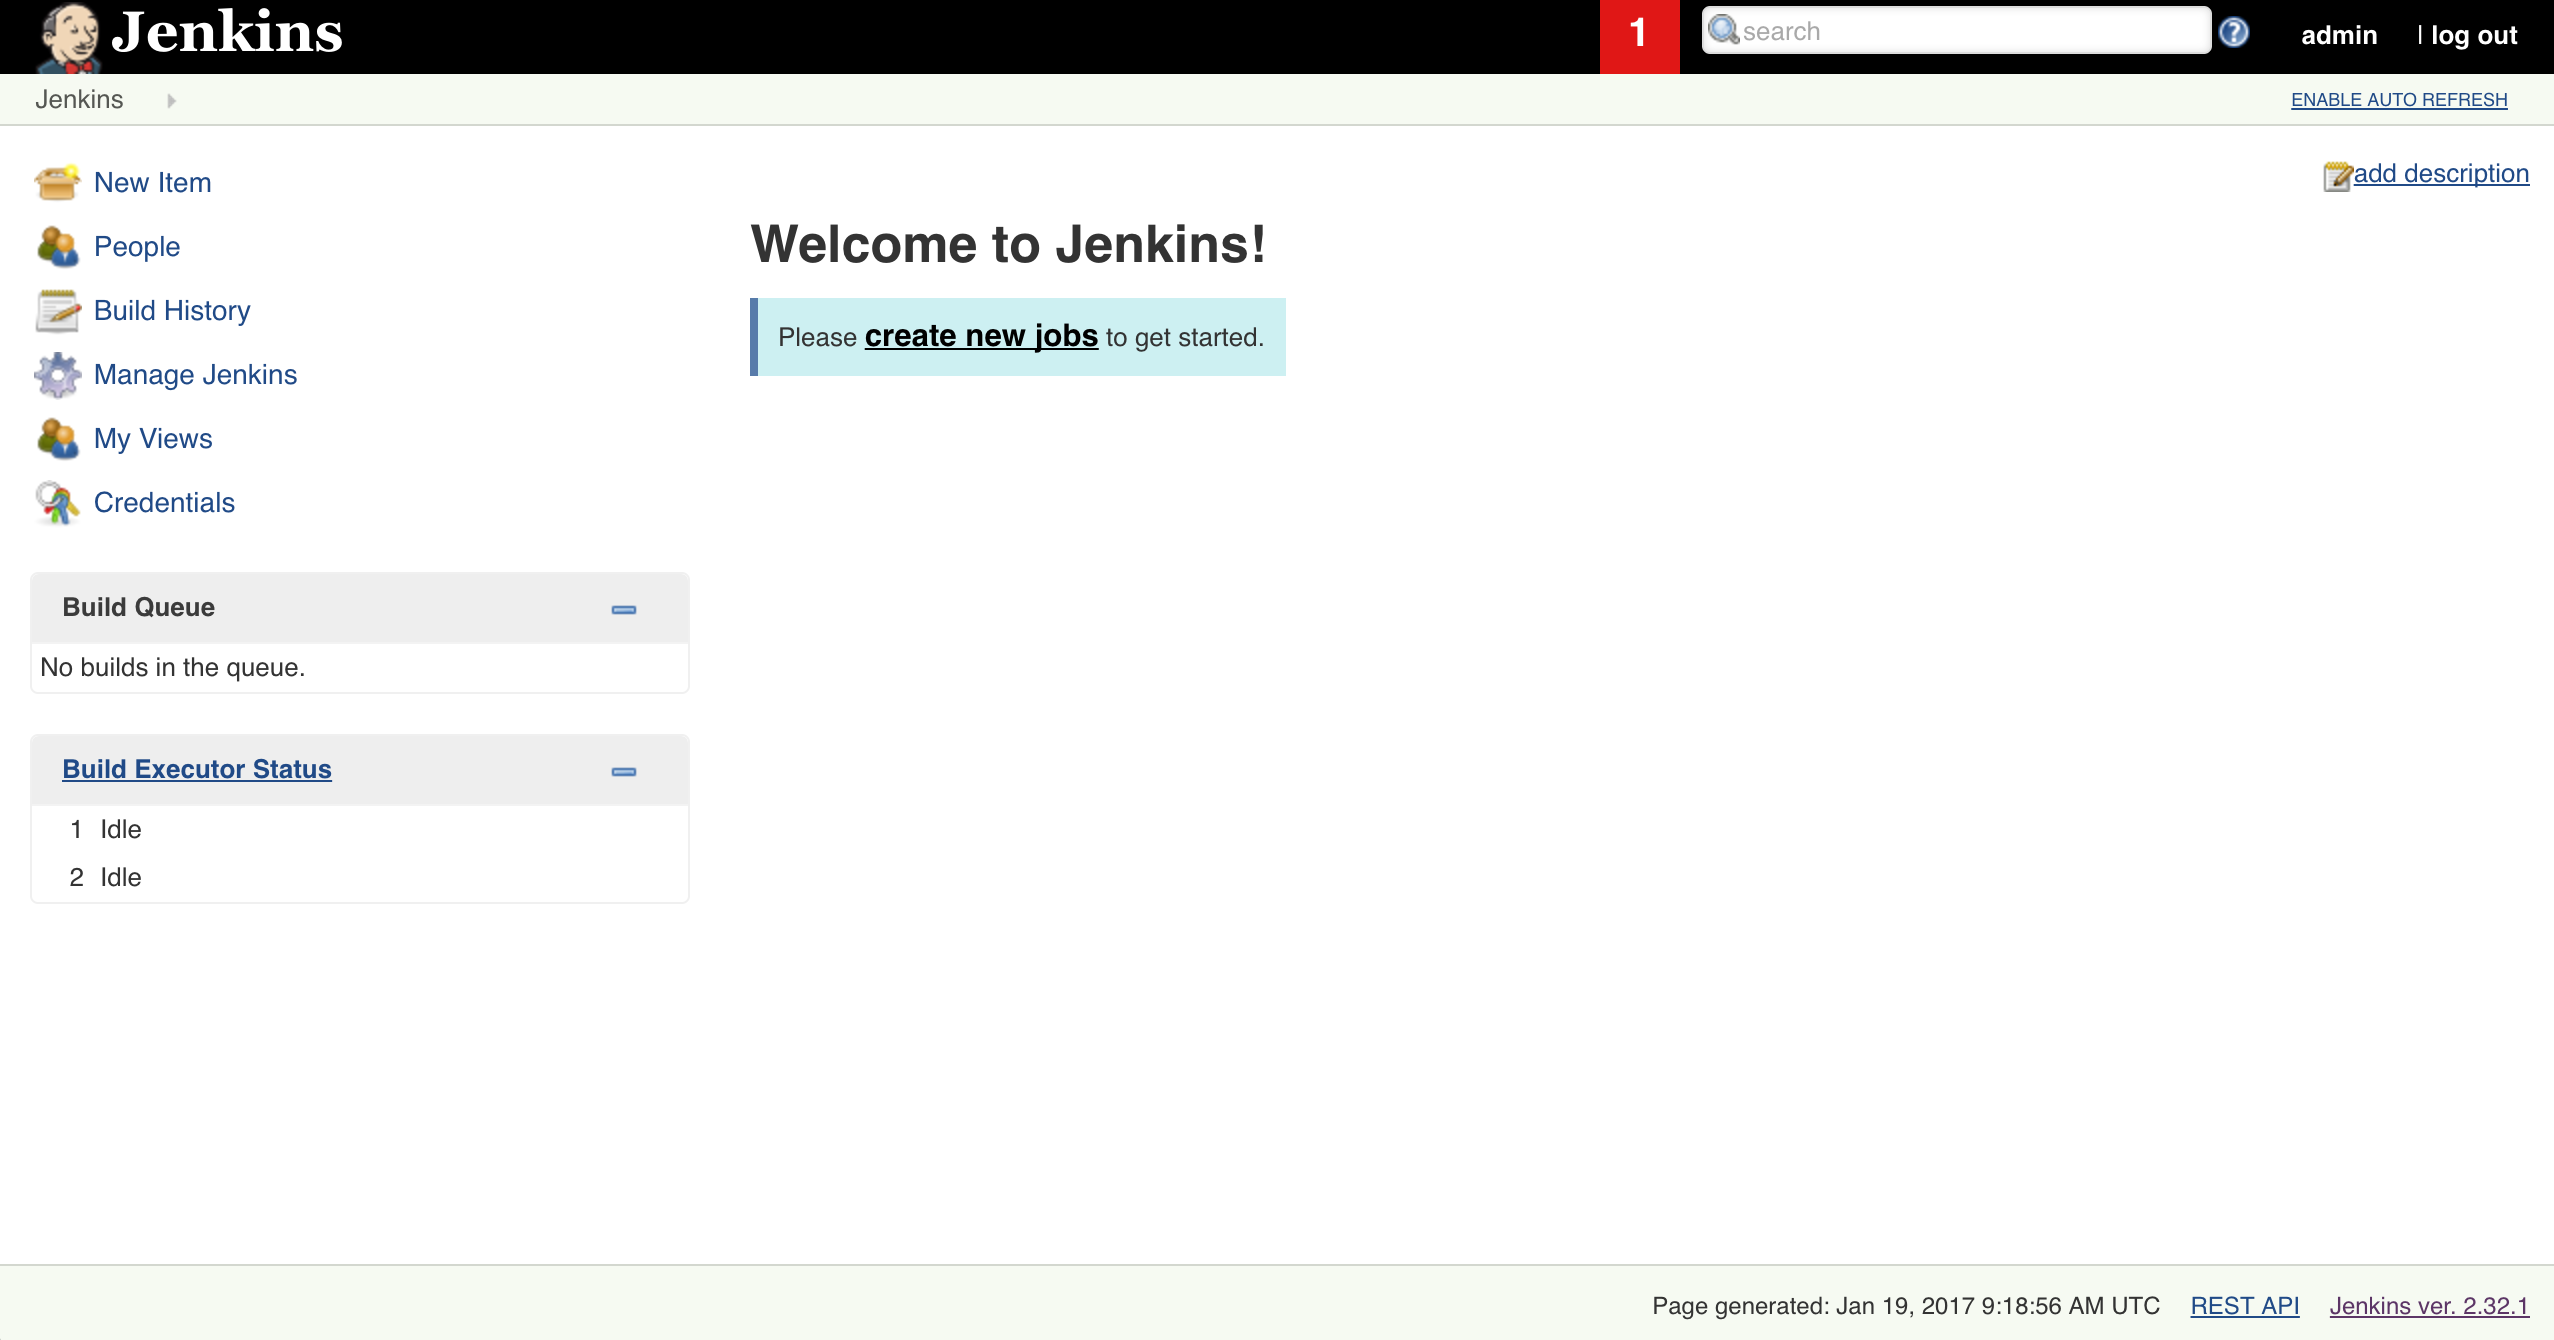
\includegraphics[width=0.8\textwidth]{grafiken/jenkins-04}
    \caption{Jenkins home page}
    \label{fig:jenkins-04}
\end{figure}

\section{Simile Jenkins Plugin installation}
To install Simile Jenkins plugin, we need to follow the following steps.

First, open Jenkins URL. Then click on \textit{Manage Jenkins} (figure \ref{fig:jenkins-plugin-01}).

\begin{figure}[H]
	\centering
    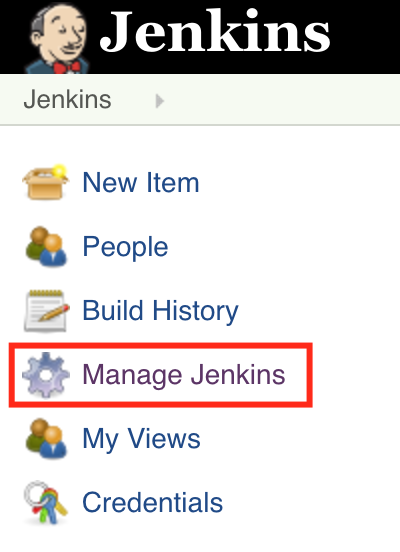
\includegraphics[width=0.25\textwidth]{grafiken/jenkins-plugin-01}
    \caption{Manage Jenkins option}
    \label{fig:jenkins-plugin-01}
\end{figure}

Then click on \textit{Manage Plugins} (figure \ref{fig:jenkins-plugin-02}).

\begin{figure}[H]
	\centering
    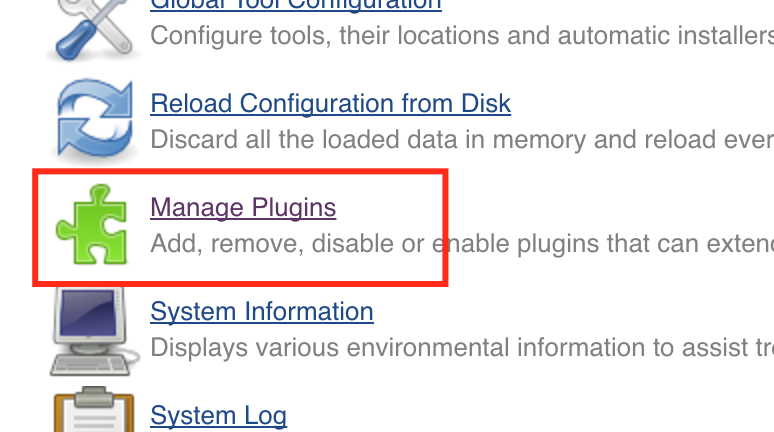
\includegraphics[width=0.5\textwidth]{grafiken/jenkins-plugin-02}
    \caption{Manage Plugins option}
    \label{fig:jenkins-plugin-02}
\end{figure}

Then go to \textit{Advanced}, scroll down until \textit{Upload Plugin} section (figure \ref{fig:jenkins-plugin-03}).

\begin{figure}[H]
	\centering
    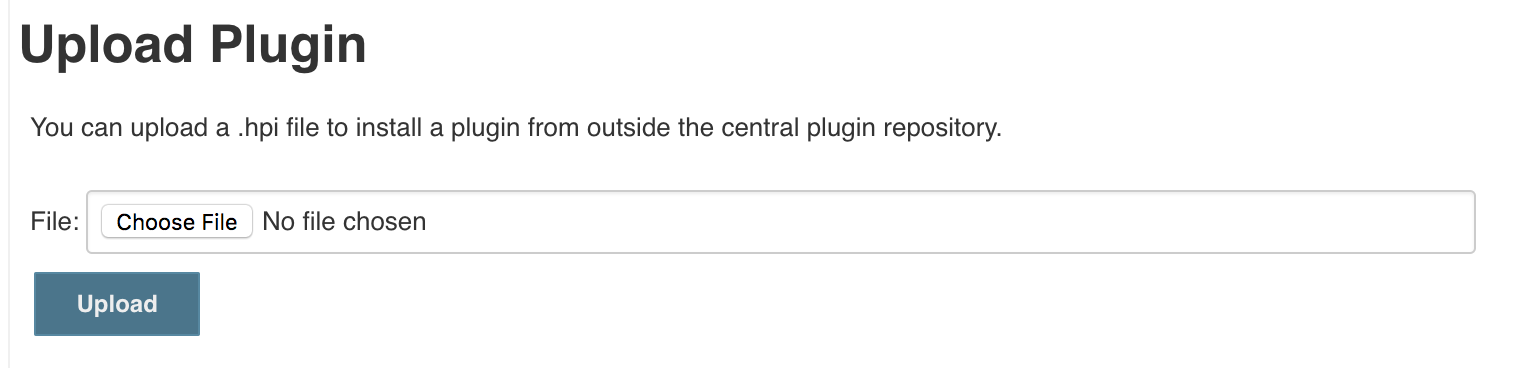
\includegraphics[width=0.9\textwidth]{grafiken/jenkins-plugin-03}
    \caption{Upload Plugin section}
    \label{fig:jenkins-plugin-03}
\end{figure}

There click on choose file and select the hpi file \textit{simile-jenkins-plugin.hpi} provided with the CD.